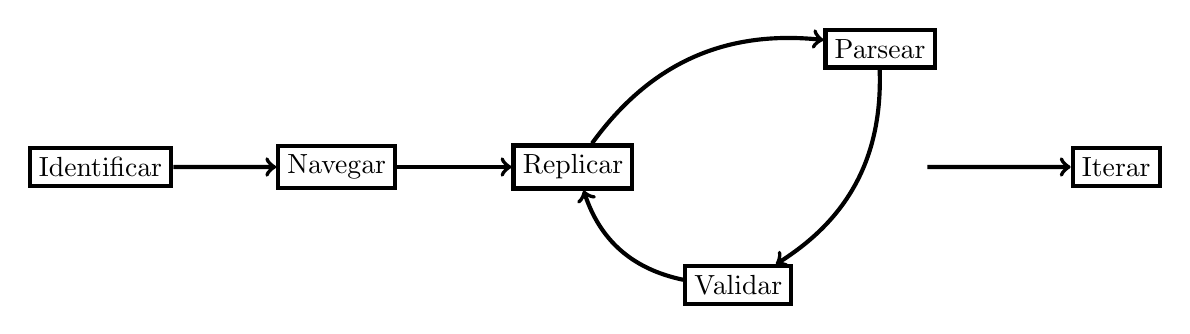
\begin{tikzpicture}[scale = 3, line width = 1.5pt]
\draw
    (1,1) node[ draw](a1){Identificar}
    (2,1) node[ draw](a2){Navegar}
    (3,1) node[ draw](a3){Replicar}
    (4.3,1.5) node[ draw](a4){Parsear}
    (3.7,0.5) node[draw](a5){Validar}
    (5.3,1) node[ draw, line width = 1.5](a6){Iterar};
    
    \draw [->] (a1) -- (a2) node[midway,below] {};
    \draw [->] (a2) -- (a3) node[midway,above] {};
    \draw[->] (4.5,1) -- (a6);
    
    \path[->] (a5) edge [bend left = 30] node[left, red] {} (a3);
    \path[->] (a3) edge [bend left = 30] node[left, red] {} (a4);
    \path[->] (a4) edge [bend left = 30] node[left, red] {} (a5);
                                                                                                                                                                                                                                                                                                                                                                                                                                                                                                                                            
\end{tikzpicture}
